\chapter{Simple Robot Formation}

\paragraph*{}
This chapter records the exploratory endeavors into the realm of swarm robotics path planning in an attempt to build a formation around an "object". A brief recapitulation of the reason we require an object is because our end goal is to perform collective transportation using swarm robotics.

\paragraph*{}
In the process of building a swarm formation, computations for the desired coordinates where the swarm units should be moving to (later referenced as \textbf{"target coordinates"}), and the desired path the members can take in order to move towards the goal are essential. The key parameters for this calculation include: the \textbf{radius} where the swarm should place itself around the object, swarm fleet \textbf{member count}, \textbf{current coordinates} for the swarm, and target \textbf{object coordinates}.

\paragraph*{}
The member count is a vital initial point since it will be used to compute the angle \(\theta\) between each set of target coordinates using the following formula:

\[\theta = (2\pi / n) * i\]

\begin{description}
    \item[where:]
    \item \(\theta\) = angle between each set of target coordinates (in radians)
    \item \(n\) = swarm system member count
    \item \(i\) = member identifier (e.g. 0 to 4 for a swarm fleet of 5 members)
\end{description}

\paragraph*{}
Currently, the formation is determined by utilizing a given radius for the swarm robotic members to attempt to surround. In accordance with the member count providing the angle, the individual target coordinates for each robot can be calculated using an adaptation from the Pythagorean Theorem. 

\[x' = x + rcos\theta\]
\[y' = y + rsin\theta\]

\begin{description}
    \item 
    \item[where:]
    \item \((x, y)\) = robot's present coordinates
    \item \((x', y')\) = target \((x, y)\) coordinates
    \item \(r\) = radius
\end{description}

\paragraph*{}
The target coordinates at this stage would often result in floats; therefore, it is necessary to round the numbers and record the margins of error to snap the coordinates to a grid system. With the resulting calculation of the target coordinates, it is sufficient to proceed to the next stage, which is \textbf{path planning}. The path planning algorithm follows a simple \textbf{"Avoid paths that cause conflicts, but if all paths cause conflicts, pause before continuing"} rule. Hence, recording the paths and the timestep the movement will happen is crucial. The algorithm is presented in Algorithm \ref{alg:path-planning-algorithm}.

\paragraph*{}
Alongside the attached algorithm, the console output for the functional instance of the algorithm is also provided. As can be seen, during the intended movement for robot2 and robot3, there is a conflicting movement in \textit{timestep 2} at the \textit{coordinates (3, 3)}. Therefore, robot3 halts for a single timestep before continuing. This is designed so that robots will not take unnecessary detours and create environmental variabilities.

\paragraph*{}
Moreover, The current implementation of the path planning algorithm also takes into account the presence of obstacles presented by the localization and object detection modules as input. The cases for obstacle appearance and avoidance can be divided into two main categories: obstacles appearing at the \textbf{turning} location while heading to the destination, and obstacles appearing while heading \textbf{straight} towards a destination.

\paragraph*{}
Obstacles appearance during turning can also be considered as the them appearing on a different axis compared to the ongoing movement (robot moving along the x axis, obstacles appear while turning onto the y axis, vice versa). Obstacles encountered this way can be tackled by continuing movement by a single step in the same direction as its ongoing movement, then computing the path as per the usual method. For visualization purposes, this case has been portrayed in Figure \ref{fig:obstacle-avoidance-case-1}.

\begin{figure} [H]
    \centering
    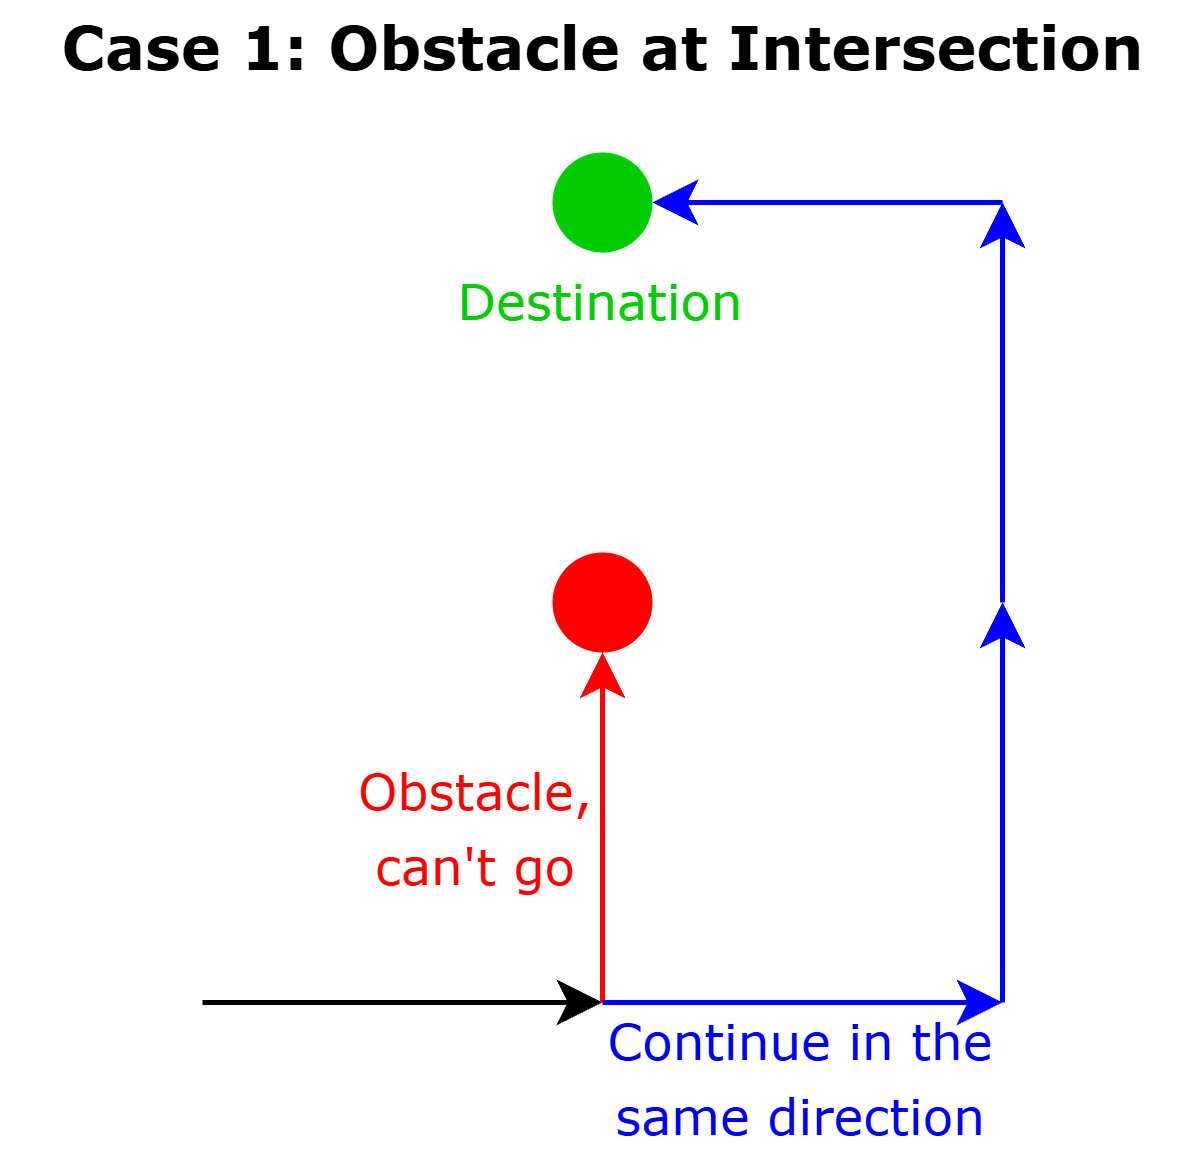
\includegraphics[width=0.55\linewidth]{assets/images/formation/obstacle-avoidance-case1.png}
    \caption{Obstacle Avoidance Case 1: Obstacle during Turning}
    \label{fig:obstacle-avoidance-case-1}
\end{figure}

\paragraph*{}
The other case for obstacle appearance can be considered as one where it coincides with the line of movement the robot is currently ongoing (robot moving along the x axis, obstacles appear along that x path). This case can be handled by "going around" the obstacles, appending movements that go around the obstacles both in the positive and negative directions, and continuing the existing path planning algorithm. Figure \ref{fig:obstacle-avoidance-case-2} illustrates the case and the proposed solution.

\begin{figure} [H]
    \centering
    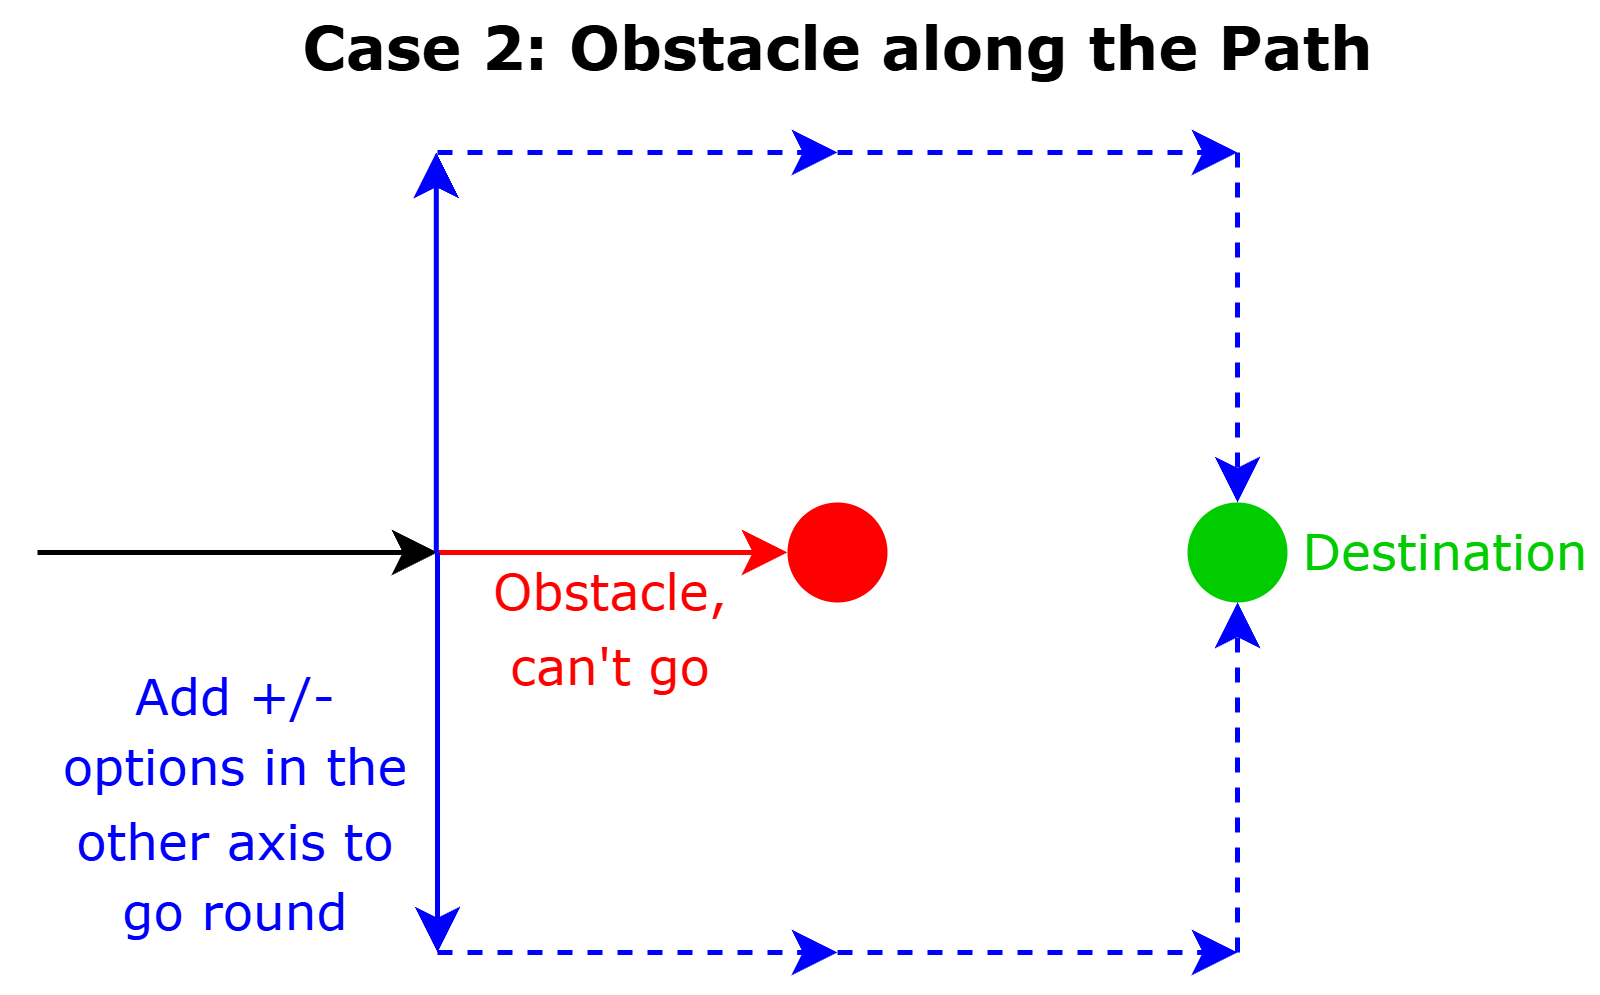
\includegraphics[width=0.75\linewidth]{assets/images/formation/obstacle-avoidance-case2.png}
    \caption{Obstacle Avoidance Case 2: Obstacle along the Current Path}
    \label{fig:obstacle-avoidance-case-2}
\end{figure}

\begin{algorithm} [H]
    \caption{Path Planning Algorithm}
    \label{alg:path-planning-algorithm}
    \begin{algorithmic}
        \STATE $\Delta x = (x_t - x_s)$ 
        \STATE $\Delta y = (y_t - y_s)$ \\
        \COMMENT{where subscript \textit{t} stands for target and subscript \textit{s} stands for start}
        \STATE $x_c =$ \FALSE
        \STATE $y_c =$ \FALSE \\
        \COMMENT{where subscript \textit{c} represents correct positions}

        \WHILE{$x_c \neq$ \TRUE $ $ \AND $y_c \neq$ \TRUE}
            % Compute possible movement options
            \IF{$\Delta x > 0$}
                \STATE $x' = x + 1$
            \ELSIF{$\Delta x < 0$}
                \STATE $x' = x - 1$
            \ELSE
                \STATE $x_c \leftarrow$ \TRUE
            \ENDIF
            \STATE $movementOptions \leftarrow (x', y)$ \COMMENT{new x, original y} \\
            \COMMENT{movementOptions is a collection of possible movements for the robot}
            \IF{$\Delta y > 0$}
                \STATE $y' = y + 1$
            \ELSIF{$\Delta y < 0$}
                \STATE $y' = y - 1$
            \ELSE
                \STATE $y_c \leftarrow$ \TRUE
            \ENDIF
            \STATE $movementOptions \leftarrow (x, y')$ \COMMENT{original x, new y}

            % Prevent collisions
            \FORALL{$movementOption \in conflictMap$}   
                \STATE $movementOptions - movementOption$
            \ENDFOR \\
            \COMMENT{conflictMap is a record of steps and paths from other robots to avoid collisions}
            
            % Avoid obstacles
            \FORALL{$movementOption \in obstacles$}
                \IF{$movementOptionDir \neq prevMovementDir$} 
                    \STATE $movementOptions \leftarrow (x, y) + prevDir$ \\
                    \COMMENT{continue moving in same direction}
                \ELSIF{$movementOptionDir = prevMovementDir$}
                    \STATE $movementOptions \leftarrow (x, y) + !prevDir$
                    \STATE $movementOptions \leftarrow (x, y) - !prevDir$ \\
                    \COMMENT{go around the obstacle}
                \ENDIF
                \COMMENT{movement in different/same axis}
            \ENDFOR \\
            \COMMENT{obstacles are from localization and object detection}
            
            % Choosing movement
            \IF{$len(movementOptions) = 0$}
                \STATE $chosenMovement \leftarrow (x, y)$ \COMMENT{stay in place}
            \ENDIF
            \STATE $chosenMovement \leftarrow movementOptions[0]$ \COMMENT{choose first movement}
            
        \ENDWHILE
    \end{algorithmic}
\end{algorithm}
